\vspace{-3cm}\chapter{实验3. 长度n的子序列最大乘积}

\section{3.1 题目}
\textbf{从文件中输入}一个数字序列字符串,计算给定的长度\lstinline{n}的子序列中的最大乘积值。

例如:如果输入“1027839564”,指定长度为3的最大子序列乘积值为 $270 = 9\times 5\times 6$;
指定长度为5的最大子序列乘积值为$7560=7\times 8\times 3\times 9\times 5$。

备注:
\begin{enumerate}
    \item 数字序列字符串的最大长度\lstinline{maxLength}的范围为:[1……1000];
    \item \lstinline{n}的取值范围为[1……\lstinline{maxLength}-1];
    \item 程序要注意处理边界情况;
    \item 程序的输入数据必须从文件中读取。
\end{enumerate}

下图为一个长度为1000的字符串数字序列,在这个序列中,长度为4的最大子序列乘积为 $5832 = 9\times 9\times 8\times 9$. 
\begin{figure}[H]
    \centering
    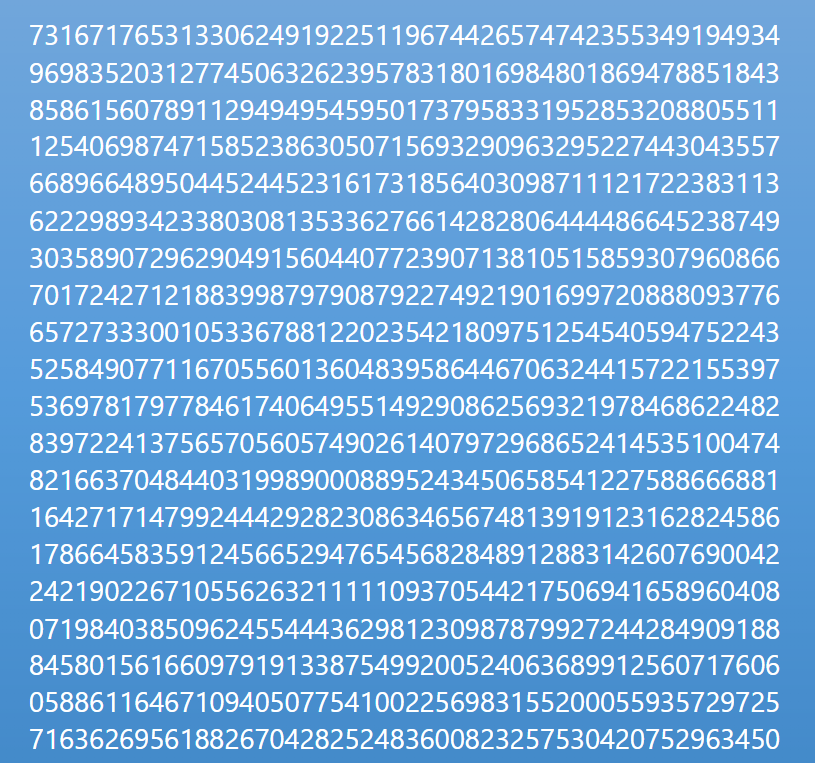
\includegraphics[width = 0.8\textwidth]{../pic/3/3.0.png}
\end{figure}

\section{3.2 思路分析}

题目本身很简单,解决和验证思路可以分为三部分
\begin{enumerate}
    \item \textbf{数据输入}. 
        \begin{itemize}
            \item 题中要求从文件输入,我们将数据存放在input文件夹的input3.txt中;
            \item 考虑到数据的长度,只能以字符串的形式输入,并通过Problem1中提到过的库函数以数组的方式处理数据。
        \end{itemize}
    \item \textbf{算法设计}. 只需要从第[0……n-1]位开始向后逐位扫描即可,但考虑到n位数相乘可能大于int甚至long类型的边界,综合
        考虑并查阅资料后,决定采用\lstinline{Math}库里的\lstinline{BigInteger}这个类. 下面对未采用的优化方案做出解释。
        \begin{itemize}
            \item 高精度. 即用\lstinline{String}模拟高位数乘法的过程。而实际上\lstinline{BigInteger}类已经帮我们内部实现了这一点,
                而且配有丰富的函数和数值优化,这一定是比我们自己写更快更方便的。
            \item 记忆组中的最小值,如果下一个比这个小就可以直接跳过。这一步看似优化了一步,实际上增加了比较的环节,从算法复杂性分析来看
                并没有优化。
        \end{itemize}
    \item \textbf{数据测试}. 本题思路简单,用题中所给数据验证即可
\end{enumerate}

\section{3.3 代码展示}

为了便于验证,用一个循环来模拟不断查询新的最大子序列

\lstinputlisting[
    language = Java,
    caption = {\bf Problem3.java}
    ]{../../../ProblemSet/src/Problem3.java}

\section{3.4 结果展示}

输入数据采用题目中的“1000位数据”,并设置三种长度

\begin{figure}[H]
    \centering
    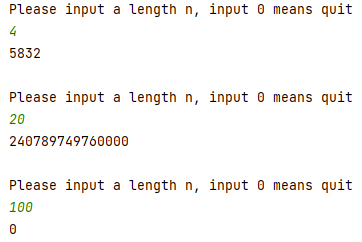
\includegraphics[width = 0.4\textwidth]{../pic/3/3.1.png}
\end{figure}

\section{3.5 总结与收获}

第一次看到本题时我想到了3.2中所写的一些思路,苦恼于怎么优化其时间复杂度以及优雅地写出来。
并不知道也没有打算使用BigInteger但后来认真分析,查阅JDK的官方文档和BigInteger的实现原理后
意识到BigInteger这个类的便捷性和性能远比自己写的好,

“如果你不知道为什么要优化,那这样的优化毫无意义(not make sense at all)” 

\rightline{—— Professor.Weaver (UC.Berkeley)}